% !TEX root = ..\main.tex
\chapter{State-of-the-Art}
This chapter presentes topics which are relevant to this project. Section 2.1 looks into technical debt with its definitions, types etc. Section 2.2 looks into embedded systems and some of the challenges with it. Section 2.3 presents 


\section{Technical Debt}
The concept of technical debt was first introduced by Ward Cunningham in 1992 to communicate the problem with non-technical stakeholders\cite{p29-cunningham}. The concept was used to describe the system design trade-offs that are made everyday. In order to deliver business functionality as quickly as possible, \textit{'quick and dirty'} decisions leading to technical debt had to be made, which affect future development activities. Cunningham further describes technical debt as \textit{"shipping first time code is like going into debt. A little debt speeds development as long as it is paid back promptly with a rewrite"}. As time goes, technical debt accumulates interest leading to increased costs of a software system\cite{p31-guo,p35-klinger}. However, not all debts are necessarily bad. A small portion of debt might help developers speed up the development process in short term\cite{p31-guo}. 


%% The costs of technical debt
\begin{figure}[ht!]
	\centering
	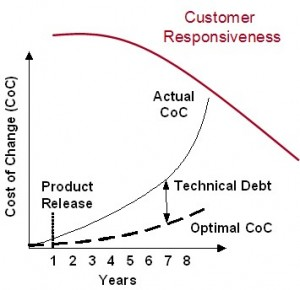
\includegraphics[width=0.8\textwidth]{images/techdebtCurve.jpg}
	\caption{The Technical Debt Curve\cite{jim-highsmith}}
	\label{fig:techDebtCurve}
\end{figure}

Figure \ref{fig:techDebtCurve} illustrates what happens as technical debt grows over time within a software product. Once we are on the far right of the curve, all choices are hard. The software controls us more than we control it.

%%%

\subsection{Types of Technical Debt}
McConnell describes TD as: \textit{a design or construction approach that is expedient in the short term but that creates a technical context in which the same work will cost more to do later than it would cost to do now (including the increased cost over time)}. He further splits the term into two categories based on how they are incurred, intentionally or unintentionally\cite{url-mcconnell}. The unintentional category includes debt that comes from doing a poor job. For example, uninntentional debt might be when a junior software developer writes bad code due to lack of knowledge and experience. Intentional debt occurs when an organization makes a decision to optimize for the present rather than the future. An example is when the project release must be done on time, or else there will not be a next release. This leads to bad decisions, like taking a shortcut to solve a problem, and then reconcile the problem after shipment

Fowlers presents a more formal explanation of how technical debt can occur\cite{url-fowler}. He categories technical debt into a quadrant with two dimensions, which he calls the \textit{"Technical Debt Quadrant"}. As seen in the Figure \ref{fig:techDebtQuad}, the debt is grouped into four categories: 

\begin{figure}[ht!]
	\centering
	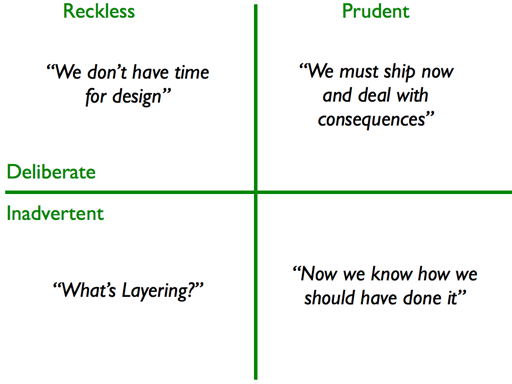
\includegraphics[width=0.8\textwidth]{images/techDebtQuadrant.png}
	\caption{Technical Debt Quadrant}
	\label{fig:techDebtQuad}
\end{figure}

\begin{itemize}
	\item \textbf{Reckless/Deliberate debt}: The team feels time pressure, and takes shortcuts intentionally without any thoughts on how to address the consequences in the future.
	\item \textbf{Reckless/Inadvertent debt}: Best practices when it comes to code and design is ignored, and a big mess in the codebase is made.
	\item \textbf{Prudent/Deliberate debt}: : The value of taking shortcuts is worth the cost of incurring debt in order to meet a deadline. The team is aware of the consequences, and has a plan in place to address them in the future. 
	\item \textbf{Prudent/Inadvertent debt}: Software development process is as much learning as it is coding. The team can deliver a valuable software with clean code, but in the end they might realize that the design could have been better.
\end{itemize}

Krutchen divides technical debt into two categories\cite{krutchen}. Visible debt that is visible for everyone. It containts elements such as new functionality to add and defects to fix. Invisible is the other category, debt that is only visible to software developers. Figure \ref{fig:techDebtLandscape} shows a map of the "technical debt landscape" which helps us to distinguish visible and invisible elements. On the left side of Figure \ref{fig:techDebtLandscape}, TD mostly affects the evolvability of the software system, while on the right it mainly affects maintainability.

\begin{figure}[ht!]
	\centering
	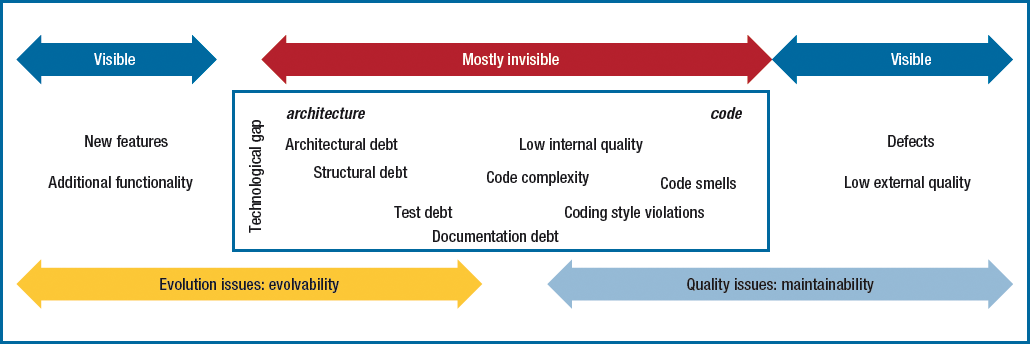
\includegraphics[width=1.0\textwidth]{images/techDebtLandscape.png}
	\caption{Technical Debt Landscaape}
	\label{fig:techDebtLandscape}
\end{figure}

\subsection{Comparison with financial debt}
Technical debt has many similarities to financial debt\cite{p50-allman,Zazworka:2011:PDD:1985362.1985372}:
\begin{itemize}
	\item You take a loan that has to be repaid later
	\item You usually repay the loan with interest
	\item If you can not pay back, a very high cost will follow. For example, you can loose your house or car.
\end{itemize}

Technical debt is in a way similar. Like financial debt, technical debt accrues interest over time which comes in the form of extra effort that have to be dedicated in future development because of bad choices\cite{p31-guo,p35-klinger}. You can choose to continue paying the interest, or you can pay down the debt by refactoring the code or system into something better which reduces interest payments in the future\cite{url-fowler}. If the debt is not repaid, development might slow down, e.g, due to poor maintainability of the code. This can lead to software project failure and you might go bankrupt\cite{p50-allman}. There are some differences between financial and technical debt as well. The debt has to be repaid eventually, but not on any fixed schedule\cite{p50-allman}. This means that some debts may never have to be paid back, which depends on the interest and the cost of paying back the debt\cite{foser076-brown}. 

Technical debt is not only about bad code design. In practice, it's much more than that. Example on interests might be lower pace of development, low competitiveness, security flaws on the system, loss of developers and their expertise, poor internal collaboration environment, dissatisfied customers and loss of market share\cite{p50-allman}.


\subsection{Causes and effects of technical debt}
Technical debt is connected with many different aspects in the software development process, like documentation debt, requirements debt, architecture debt etc\cite{Falessi:2015:FRI:2797433.2797462}. 

%While financial debt occus from deliberate actions of taking a loan, technical debt may be caused by several factors. Antares categories these factors into four groups:
%\begin{itemize}
%	\item Work processes: Software development methology, can some tasks be automized (with a deploy script), is tests written after bug fixing, do you map and document shortcuts you take, is there any plans for techincal debt management later, is it important to implement new functionality or to make sure that the existing ones work propertly?
%	\item People (knowledge and capacity): Do you need some individuals to finish a task, Do you have the right people for the job, is enough training given to new people, what happens if you need someone who's on vacation/change project/is sick or something. You should keep this in mind and make a plan on how knowledge is transferred. Techcnical debt can be the reason for poor motivation and productivity which causes you to work poorly. 
%	\item Technology: Is solutions hard to integrate with other solutions, is all the systems out there compatible with newer technology, is there any outdated or duplicated code in the system, is all the systems secure, is the solutions old, or user friendly, is there some code which is hard to maintencance. 
%	\item Collaboration in the organization: Commuinication between developers and requirement people. You often get a list with requirements, is the list understandable? Do we work with a backlog with tasks that should have been solved long time ago, but not which is not "actual" now?
%\end{itemize}
%Developers might not care about the product because they don't feel that they "own" what's being made. They get told what do to, but not more than that. Can't make requirements.


%Operating technical debt might be to maintenance and manage existing code rather than implementing new functionality. It is important to keep track of the technical debt, and incur interest payments, before it makes troubles for you. Do do that, you could for example set up a plan for repayment which tells you something about how the debt shall be repayed. Scrum can be used to do this for example, where you split the repayment plan to smaller parts where you estimate and prioritize tasks. It is important to remember that taking too much loan might cause problems. As mentioned ealier, technical debt can be seen as taking a financial loan according to Cunningham. The loan has to be repaid with interests. Technical debt uses time and effort as repayment. It is acceptable to take a loan, but it should be controlled. Do not take loan than what you are able to handle. Think with your head.

%Main developers behind a software project aren't the one who usually maintain the code. Companies often has policies where they transfer a project to new developers after the development phase is over. The reasons could be to save money, or that the new developers might work more. These maintenance people often haas to repay the debt. The main developers gets awarded for their implementation speed rather than thinking on maintanence and evolution. They can often be placed on new projects before the debt has to be paid back, making them unavaiable for a period. Too few systems also has TODO or FIXME comments in their source code.

Klinger et al.\cite{p35-klinger} carried out an industrial case study at IBM where four technical architechts with different backgrounds were interviewed and the goal was to examine how the decisions to incur debt were taken and the extent to which the debt provided leverage\cite{p35-klinger}. The study revealed that the company failed to assess the impact of intentionally incurring debt on projects. Decisions regarding technical debt were rarely quantified. There were also big organizational gaps among the business, operational and technical stakeholders, which incurred debt. Pressure from stakeholders, decisions were made without quantifications of possible impacts, an unintenional debt occuring from acquisitions, change of requirements, and changes in the market ecosystem.

Lim et al.\cite{lim-taksande} show us that technical debt is not always the result of poor developer discipline or sloppy programming. It can also include intentionals decisisions to trade off competing concerns during business pressure. They also found out that tech debt can be used in short term to capture market share and to collect customers feedback early. In the long term, tech debt tended to be negative. These tradeoffs included increased complexity, reduced performance, low maintainability, and fragile code. This led to bad customer satisfaction and extra working hours. In come cases, the short term benefits of tech debt outweighted the future costs.

Guo et al.\cite{guo2011tracking} studied the effects of technical debt by tracking a single delayed maintenance task in a real software project throughout its lifecycle, and simulated how managinc technical debt can impact the project result. The results showed that delaying the maintenance task would have almost tripled the costs if it had been done later.

Siebra et al.\cite{p247-siebra} carried out an industrial case study where they analyzed documents, emails code files, and had interviews with developers and project managers. This case lasted for six years. This study revealed that technical debt were mainly taken by strategic decisions. They also found out that using a unique specialist could lead the development team to solutions that the specialist wants and believes are correct, leading the team to incur debt. The study also identified that TD can both increase and decrease the amount of working hours.

Zazworka et al.\cite{zazworka2011investigating} studied the effects of god classes and design debt on software quality. God classes are examples on bad coding, and therefore includes a possibility for refactoring\cite{Zazworka:2011:PDD:1985362.1985372}. The results shows that god classes require more maintenance effort that include bug fixing and changes to software that are considered as a cost to software project.

Buschmann\cite{buschmann2011pay} explained three different stories of technical debt effects. In the first case, technical debt in one platform started to grow so large that development, testing, and maintenance costs started to increase dramatically, and the components were hardly usuable. In the second case, developers started to use use shortcuts to increase the development speed. This resulted in significant performance issues because an improper software modularization reflcted organizational structures instead of the system domains. It ended up turning in to economic consequences. In the third case, an existing software product experienced increased maintainenance cost due to architecture erosion. However, management analyzed that reengineering the whole software would cost more than doing nothing. This resulted in a situation where the management decided not to do anything to technical debt, because it was cheaper from a business point-of-view.

Codabux et al.\cite{p8-codabux} carried out an industrial case study where the topic was agile development focusing on techincal debt. They observed and interviewed developers to understand how technical debt is characterized, addressed, prioritized, and how decisions led to technical debt. They made two definitions of technical debt, infrastructure and automation debt. 

These studies shows that the causes and effects of technical debt are not always caused of technical reasons. It can be caused by intentional decisions that are related to business reasons. Taking some technical debt may have short-term positive effects such as time-to-market benefit. The tradeoff are economic consequences, and quality issues in the long run if TD is not paid back. The allowance of TD can facilitate software development for a while, but decrease the product maintainability in the long term at the same time. However, there are some times where short-term benefits overweight long-term costs. 

These studies also reveales that technical debt is not just related to shortcuts in code. There are several subcategories that has been defined in the literature, which is shown in Table \ref{tab:subcategories}.

\begin{table}
	\centering
	\begin{tabular}{ | p{5cm} | p{8cm} |}
	\hline
	\textbf{Subcategory} & \textbf{Definition} \\ \hline
	Architectural debt\cite{li2015systematic,p8-codabux,foser076-brown} & Architectural decisions that make compromises in some of the quality attributes, such as modifiability. \\ \hline
	Code debt\cite{li2015systematic,foser076-brown,tom2013exploration} & Poorly written code that violates best coding practices and guidelines, such as code duplication. \\ \hline
	Defect debt\cite{li2015systematic,tom2013exploration} & Defect, failures, or bugs in the software. \\ \hline
	Design debt\cite{li2015systematic,Zazworka:2011:PDD:1985362.1985372,foser076-brown} & Technical shortcuts that are taken in design.\\ \hline
	Documentation debt\cite{li2015systematic,foser076-brown,Zazworka:2013:CSE:2460999.2461005} & Refers to insufficient, incomplete, or outdated documentation in any aspect of software development.\\ \hline
	Infrastructure debt\cite{li2015systematic,tom2013exploration,p8-codabux} & Refers to sub-optimal configuration of development-related processes, technologies, and supporting tools. Lack of continious integration is an example.\\ \hline
	Requirements debt\cite{li2015systematic,Zazworka:2013:CSE:2460999.2461005} & Refers to the requirements that are not fully implemented, or the distance between actual requirements and implemented requirements.\\ \hline
	Test debt\cite{li2015systematic,Zazworka:2013:CSE:2460999.2461005,foser076-brown} & Refers to shortcuts taken in testing. An example is lack of unit tests, and integration tests.\\
	\hline
	\end{tabular}
	\caption{Technical debt subcategories} \label{tab:subcategories}
\end{table}

\subsection{Current strategies and practices for managing technical debt}
Managing technical debt compromises the actions of identifying the debt and making decisions about which debt should be repaid. Brown, Krutchen, McConnell 

Se på comparing four approaches

%Lim.et al - 4 strategies
Lim et. al found four strategiest for managing technical debt. The first strategy is to do nothing because the technical debt might never be visible to the customer. The second strategy is to use a risk management approach to evaluate and prioritize technical debt's cost and value by allocating five to ten percent of each release cycle to address technical debt. The third strategy is to include the customers and nontechnical stakeholders to technical debt decisions. The last strategy is to track technical debt using tools like a Wiki, or a backlog.

%Codabux
Codabux et al. suggests best practices such as refactoring, repackaging, reengineering, and developing unit tests to manage technical debt.

%Portifolio management (guo, zazworka (priorizing design debt investment opportunities))
Guo et. al suggest the use of portfolio managemnt for technical debt management. This approach collects technical debt to a "technical debt list" that is being used to pay the technical debt back based on its cost and value.

%Quantifying technical debt - Nugraho
Nugraho et. al proposes an approach to quantify technical debt and its interest by using a software quality assessment method. This method rates the technical quality of a system in terms of the quality characteristics of ISO9126. 

%Krutchen (define tech debt in your backlog)
Krutchen suggest listing debt-related tasks in a common backlog during release and iteration planning. Figure \ref{fig:fourColorBacklog} illustrates how these elements can be organized in a backlog. Krutchen further mentions that project backlogs often contain the green elements. The rest are seen rarely, especially the black elements, they are nowhere to be found.

\begin{figure}[ht!]
	\centering
	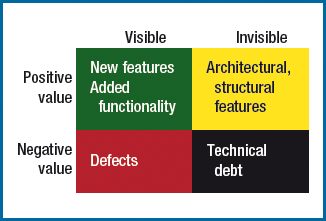
\includegraphics[width=0.8\textwidth]{images/fourColorBacklog.png}
	\caption{The colors reconcile four types of possible improvements.}
	\label{fig:fourColorBacklog}
\end{figure}



%Allman

%A systematic mapping study on tech debt and its management


%To pay or not to pay



SonarQube is an open source application for quality management. It manages results of various code analysis tools, and is used to analyze and measure a projects technical quality. The technical debt is computer based on the SQALE (Software Quality Assessment based on Lifecycle Expectations) methodology. SQALE is a method for assessing technical debt in a project. It is based on tools that analyze the source code of the project, looking at different types of errors such as mismatched indentation, and differnet naming conventions. Each error is assigned a score based on how much work it would take to fix that error. The analysis gives a total sum of technical debt for the entire project.



\subsection{Organizational debt}
While technical debt is known problem, there's one more type of debt which can be accrued on a compandy-wide level. This type of debt is called organizational debt. Organizational debt is all about people and culture compromises made to \textit{'just get it done'} in early stages of a startup, preventing a company from running smoothly\cite{steve-blank}. When things should be going great, organizational debt can turn a growing company to a nightmare. Growing companies needs to know how to recognize and refactor organizational debt. 

Some of the causes behind organizational debt might be:

\begin{itemize}
	\item Training the new hires, both culture and specific tasks
	\item Retain existing hire by doing something for them. Many doesn't get promoted. New hire might get a better posistion than existing hire who has been there from the start.
\end{itemize}

Sometimes, the employees gets awarded by good building, new furnitures, and compensation for executive staff. However, that isn't enough. Think about existing employees who's been there from the start. You might end up loosing qualified people who's spent years building up the company, but not compensated for it. Top-down approach is focused too much. Think about the bottom employees.They have the inistituinal knowledge and hard-earned skills.

When new people got hired, the ones who could train them about the company culture and how to do their specific tasks is the old employees who's being underpaid. They will look for another job. No one would be able to train the new people then. Giving compensation in form of stock vesting, insurance benefits, movie nights etc isnt enough as everyone gets it. Do something for the employees who's been there for a long time.

Refarocting might be important in order to reduce the organizational debt. Write plan for managing new wave of hires before hiring them. Sometimes, you'll also need to think about what you will have to do if you're about to loose a key employee. Is it worth to replace employees who hold critical knowledge? Put together an expence budget using the current employee salaries. See who's important. Identify the one they wanted to keep and upgrade them. Some employees might not be that important as welll as they might be a performance problem for the whole organization. Need to look at the company culture as well, does it take into account of the new size and stage of the organization? What have the company achieved, what are the key elements that have made it great so farm, are they same of different. Think about the customer too. Does we talk to the customer, or does the customer talk to us. Also, keep in mind that an adivosory board of other CEOS who've been through the early stages might be good. Failure to refactor might kill a growing company\cite{steve-blank}.

Some examples on organizational debt:
\begin{itemize}
	\item Different departments solving the same problems might use differnet methologies and tools. Difficult to see similarities in order to address company-wide issues.
	\item Creation of processes and implement solutions which seems great at first, but didnt address the root casue of the issue and ending up creating more problems.
	\item Time constraints, solving a problem in less-than-ideal manner this time. This manner is repeated because no one remember that the first time was intended to be one-off situation.
\end{itemize}

%%%%%%%%%%%%%%%%%%%%%%%%%%%%%%%%%%%%%%%%%%%%%%%%%%%%%%%%%%%%%%%%%%%%%%%%%%%%%%%%%%%%%%

			% SOFTWARE LIFECYCLE

%%%%%%%%%%%%%%%%%%%%%%%%%%%%%%%%%%%%%%%%%%%%%%%%%%%%%%%%%%%%%%%%%%%%%%%%%%%%%%%%%%%%%%

\section{Software Lifecycle}
Software lifecycle are the phases a software product goes through between its conceived and when its no longer available for use. There are five general groups of related activities in the software lifecycle according to IEEE Standard for Developing Software Life Cycle Processes\cite{159431}. 

\begin{enumerate}
	\item The first group is project management. Every software lifecycle starts with the project initiation. Project planning, and project monitoring and control are two other, necessary activities withing this group for each project iteration. 
	\item The second group is of pre-development. This group consists of activities that needs to be performed before the software development phase. Concept exploration is a good example of such acitity. 
	\item The third group is the development itself. It includes the activities that must be performed during the development.
	\item The fourth group is of post-development. It includes activities to be performed after development to enchance the software project. The retirement activity involves removal of the existing system from its active support by ceasing its operation or support, or replacing it with a new system or an upgraded version of the exisiting system. 
	\item The final group is called integral. This group consists of activities that are necessary to ensure successful completion of a project. These activities is seen as support activities rather than activities that are directly oriented to the development effort.
\end{enumerate}

\subsection{Software development life cycle and methodologies} % (fold)
A software development process or a software development lifecycle is defined as the process by which user needs are translated into a software product\cite{radatz1990ieee}. The process involves translating user needs into requirements, transforming requirements into design, implementing design into code, testing the code, and sometimes, installing and checking out the software for operational use.

A software development methodology is defined as a framework to structure, plan, and control the software development process. Many software development methodologies exists, and the basic lifecycle acitivites are included in all lifecycle models, often in different orders. The difference is in terms of time to release, risk management, and quality. The models can be of different types, but they are usually defined as traditional and agile software development methodologies.

Traditional software development methodologies are based on a sequential series of steps. It usually starts with elicitation and documentation of a complete set of requirements, followed by architecture and high level design, development, testing, and deployment. The most well-known of these traditional software development methodologies is the Waterfall method.

Using sequential design processes in software development processes to build complex, intensive systems is often a failure\cite{p50-allman}. Requirements are specified at the beginning of the software development process, and the remaining software development activities have to follow the initial requirements. This kind of model is not appropiate to use for software where technology and business requirements always change. 

%This is why agile methods was made, where change and feedback is important. One of the benefits is the ability to quickly release new functionality. However, one of the problems with agile methods is that developers often wants to focus on implementing new fucntionality, which results in poor focus on design, code quality, testing, which again leads to technical debt.  

To address the challenges posed by traditional methods, agile methods were developed as a set of lightweight methods. This methods tries to deal with collaboration in a way that promotes adaptive planning, early delivery, and continious improvement, making the development phase faster and more flexible regarding changes. There are four values that defines agile software development: 

\begin{itemize}
	\item Individuals and interactions over processes and tools
	\item Working software over comprehensive documentation
	\item Customer collaboration over contract negotiation
	\item Responding to change over following a plan
\end{itemize}

Lean, Scrum

\begin{figure}
	\centering
	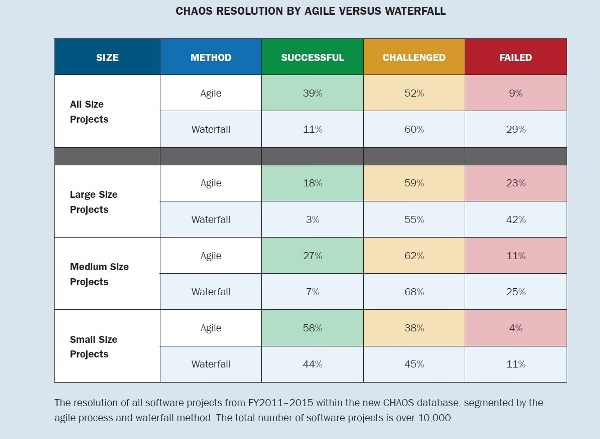
\includegraphics[width=0.8\textwidth]{images/Agile-Waterfall-Success-Failure-Rates.jpg}
	\caption{The CHAOS Manifesto, The Standish Group 2012}
	\label{fig:agileWaterfallSuccessFailureRates}
\end{figure}


%%%%%%%%%%%%%%%%%%%%%%%%%%%%%%%%%%%%%%%%%%%%%%%%%%%%%%%%%%%%%%%%%%%%%%%%%%%%%%%%%%%%%%

			% SOFTWARE ARCHITECTURE

%%%%%%%%%%%%%%%%%%%%%%%%%%%%%%%%%%%%%%%%%%%%%%%%%%%%%%%%%%%%%%%%%%%%%%%%%%%%%%%%%%%%%%
\section{Software Architecture}
Bass, Klements and Kazman\cite{Bass:2012:SAP:2392670} defines software architecture as following: 

\begin{displayquote}
The software architecture of a system is the set of structures needed to reason about the system, which compromise software elements, relations among them, and properties of both.
\end{displayquote}

The architecture of a software is one of the most important artifacts within the systems life cycle\cite{Bass:2012:SAP:2392670,knodel2006static}. Architectural design decisions that are made during the design phase, affect the systems ability to accept changes and to adapt to changing market requirements in the future. As the design decisions are made early, it will directly affect the evolution and maintenance phase\cite{Pressman:2009:SEP:1593949}, activities that consumes a big part of the systems lifespan\cite{Vliet:2008:SEP:1481475}. Software architecture can be seen from two standpoints; prescriptive and descriptive architecture. The prescriptive architecture of a system captures the design decisions made prior to the construction. This is normally called as-conceived software architecture. Descriptive architecutre describes how the system has actually been build, called for as-implemented software architecture. 

As the system evolves, it is ideal that the prescriptive architecture is modified first. In practice, the system - the descriptive architecture - is often directly modified. This can be due to developers sloppiness, short deadlines, or lack of documented prescriptive architecture. This introduces two new concepts, architectural drift and architectural erosion. Architectural drift occurs when the documents are updated according to the implementation. The software architecture ends up as an architecture without vision and direction. Architectural erosion occurs when the implementation drifts away from the planned architecture. 

The software architecture plays a vital role in achieving quality attributes.
- Availability
- Interoperability
- Modifiability
- Performance
- Security
- Testability
- Usability


%%%%%%%%%%%%%%%%%%%%%%%%%%%%%%%%%%%%%%%%%%%%%%%%%%%%%%%%%%%%%%%%%%%%%%%%%%%%%%%%%%%%%%

		% SOFTWARE MAINTENANCE AND EVOLUTION

%%%%%%%%%%%%%%%%%%%%%%%%%%%%%%%%%%%%%%%%%%%%%%%%%%%%%%%%%%%%%%%%%%%%%%%%%%%%%%%%%%%%%%
\section{Software Evolution}
Increasingly, more and more software developers are employed to maintain and evolve existing systems instead of developing new systems from scratch\cite{Sommerville:2011:SE}. Software evolution is a process that usually takes place when the initial development of a software project is done and was successful\cite{Bennett:2000:SME:336512.336534}. The goal of software evolution is to incorporate new user requirements in the application and adapt it to the existing application. Software evolution is important beacuse it takes up to 85-90\% of organizational software costs\cite{Sommerville:2011:SE}. It is also important because technology tend to change rapidly, and not following these trend means loosing business oppertunities.

Rajlich and Bennet\cite{Bennett:2000:SME:336512.336534} proposed a view of the software lifespan, as shown in Figure \ref{fig:lifespan-1}. This view divides the software lifespan into five stages with initial development as the first stage. The key contribution is to seperate the maintenance phase into an evolution stage followed by a servicing stage and phase-out stages.
\begin{description}
	\item[Initial development] produces the first version of the software from scratch.
	\item[Evolution] is the phase where significant changes to the software may be made. This could be addition of new features, correct previous mistakes, or adjust the software to new business requirements or technologies. Each change introduces a new feature or some other new property into the software.
	\item[Servicing] is the stage where relatively small, essential changes are allowed. The company considers how the software can be replaced. Legacy software is a term to describe software in this stage.
	\item[Phase-out] is the phase where software may still be used, but no further changes are being implemented. Users must work around any problems that they discover, or replace the software with something else.
	\item[Close-down] is when the managers or customers completely withdraw the system from production.
\end{description} 

\begin{figure}[ht!]
	\centering
	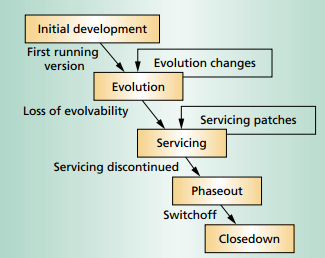
\includegraphics[width=0.8\textwidth]{images/lifespan-1.png}
	\caption{Software evolution process}
	\label{fig:lifespan-1}
\end{figure}

A variation of this process is the versioned stage model, as shown in Figure \ref{fig:lifespan-2}. When a software version is completed and released to the customer, the evolution continues with the company eventually releasing another version and only servicing the previous version. 

\begin{figure}[ht!]
	\centering
	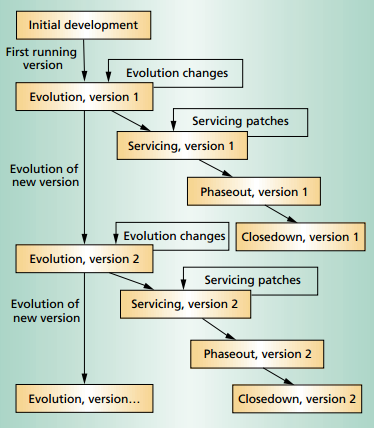
\includegraphics[width=0.8\textwidth]{images/lifespan-2.png}
	\caption{Software lifespan}
	\label{fig:lifespan-2}
\end{figure}

\subsection{Evolution processes}
Software evolution usually starts with change proposals, which may be new requirements, existing requirements that have not been implemented, or bug reports from stakeholders. The process of implementing a change goes through these stages\cite{Sommerville:2011:SE} which can be seen in Figure \ref{fig:seProcess}.

The process starts with a set of proposed change requests. The cost and impact of the change is analyzed to decide wether to accept or deny the proposed changes. If the proposed changes are accepted, a new release of the system is planned. During release planning, all proposed changes such as fault repair, adaptation, and new functionality, are considered, in order to decide which changes to implement in the next version of the system. The changes are implemented and validated, and a new version of the system is released. The process ends with a new iteration with a set of proposed change requests for the next release. 

Sometimes, things that require urgent change may appear, such as a serious system fault that must be repaired to allow normal operation. In these cases, the usual process wont be beneficial as it takes time. An emergency fix is usually made to solve the problem. A developer choose a quick and workable solution rather than the best solution. The trade-off is that the the requirements, the software design, and the code become inconsistent. As a system changes over time, it will have impact on the systems internal structure and complexity. Software evolution might cause poor software quality and erosion of software architecture over time\cite{Bass:2012:SAP:2392670}.

\begin{figure}[h!]
	\centering
	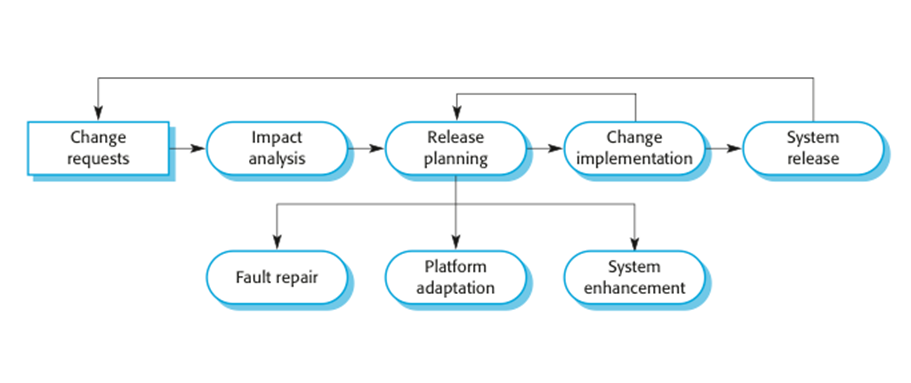
\includegraphics[width=0.8\textwidth]{images/SEprocess.png}
	\caption{Software evolution process}
	\label{fig:seProcess}
\end{figure}


\subsection{Software maintenance}
IEEE 1219 defines software maintenance as follows\cite{720567}:
\begin{displayquote}
Modification of a software after delivery to correct faults, to improve performance or other attributes, or to adapt the product to a modified environment.
\end{displayquote} 
Maintenance can be classified into four types\cite{Bennett:2000:SME:336512.336534,720567}.

\begin{itemize}
	\item Adaptive: Modification of a software product performed after delivery to keep a computer program usable in a changed or changing environment.
	\item Perfective: Modification of a software product after delivery to improve performance or maintainability.
	\item Corrective: Reactive modification of a software product performed after delivery to correct discovered faults.
	\item Preventive: Maintenance performed for the purpose of preventing problems before they occur.
\end{itemize}

According to van Vliet, the real maintenance activity is corrective maintenance\cite{Vliet:2008:SEP:1481475}. 50\% of the total software maintenance is spent on perfective, 25\% on adaptive maintenance, and 4\% on preventive maintenance. This leads to that 21\% of the total maintenance activity is corrective maintenance, the 'real' maintenance\cite{Vliet:2008:SEP:1481475}. This has not changed since the 1980s when Lientz and and Swanson conducted a study on software maintenance\cite{lientz1980software}. Their study found out that most severe maintenance problems was caused by poor documentation, demand from users for changes, poor meeting schedulment, and problems training new hires.  Some other problem areas was lack of user understand and user training, the customers did not understand how system works.

\begin{figure}
	\centering
	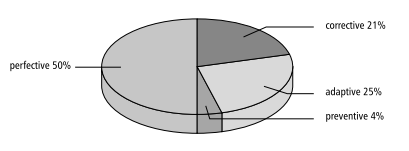
\includegraphics[width=0.8\textwidth]{images/maintenance.png}
	\caption{Distribution of maintenance activities\cite{Vliet:2008:SEP:1481475}}
	\label{fig:maintenanceActivities}
\end{figure}



%%%%%%%%%%%%%%%%%%%%%%%%%%%%%%%%%%%%%%%%%%%%%%%%%%%%%%%%%%%%%%%%%%%%%%%%%%%%%%%%%%%%%%

			% SOFTWARE REUSE

%%%%%%%%%%%%%%%%%%%%%%%%%%%%%%%%%%%%%%%%%%%%%%%%%%%%%%%%%%%%%%%%%%%%%%%%%%%%%%%%%%%%%%
\section{Software Reuse}
Software reuse is the process of using existing software artifacts, or knowledge, to create new software, rather than building it from scratch. Software reuse is a key method for improving software quality\cite{frakes1996software}. Software reuse can be specified in two directions: development for reuse and development with reuse[53][49]. Development for reuse is related to components for reuse or system generalization. Development with reuse is related to how existing components can be reused in new system.

Table \ref{tab:reusableComponents} lists several assets from a software project that can be reused\cite{frakes1996software}.

\begin{table}[H]
	\centering
	\begin{tabular}{ | l | l |}
	\hline
	1. architectures & 6. estimates \\ \hline
	2. source code & 7. human interfaces \\ \hline
	3. data & 8. plans \\ \hline
	4. designs & 9. requirements \\ \hline
	5. documentation & 10. test cases \\
	\hline
	\end{tabular}
	\caption{Reusable assets in software projects} \label{tab:reusableComponents}
\end{table}


%%%%%%%%%%%%%%%%%%%%%%%%%%%%%%%%%%%%%%%%%%%%%%%%%%%%%%%%%%%%%%%%%%%%%%%%%%%%%%%%%%%%%%

			% REFACTORING

%%%%%%%%%%%%%%%%%%%%%%%%%%%%%%%%%%%%%%%%%%%%%%%%%%%%%%%%%%%%%%%%%%%%%%%%%%%%%%%%%%%%%%
\section{Refactoring}
Design debt, a specific type of technical debt, accumulates as you write code\cite{Zazworka:2011:PDD:1985362.1985372}. This type of debt can be reduced when you refactor. Fowler defines refactoring as means of adjusting the design and architecture towards new requirements without changing the externial behaviour of a program in order to improve the quality of the system\cite{1999:RID:311424}. It is an act of improving the design of an existing system\cite{Vliet:2008:SEP:1481475}. Most of the time in spent on reducing design debt is on refactoring activities itself. These activities includes planning the design and architecture, rewriting the code, and adjusting documentation\cite{Pressman:2009:SEP:1593949}. It is believed that refactoring is one of the key methods to reduce technical debt in a system as it can be applied to code smells or at the architecture level (Lippert and Roock, 2006).  


%%%%%%%%%%%%%%%%%%%%%%%%%%%%%%%%%%%%%%%%%%%%%%%%%%%%%%%%%%%%%%%%%%%%%%%%%%%%%%%%%%%%%%

			% CONFIGURATION MANAGEMENT

%%%%%%%%%%%%%%%%%%%%%%%%%%%%%%%%%%%%%%%%%%%%%%%%%%%%%%%%%%%%%%%%%%%%%%%%%%%%%%%%%%%%%%
\section{Configuration Management}
Systems always change to cope with bugs and introduce new features. A new version of a system is created when changes are made. Dart\cite{dart1991concepts} defines configuration management (CM) as a dicipline for controlling the evolution of software systems. CM identifies every component in a project and has an overview of every suggestions and changes from day one to the end of the product. CM involves four related activities\cite{Sommerville:2011:SE}:
\begin{description}
	\item[Change management] is intented to ensure that the evolution of a system is a managed process, and to prioritize changes. Costs and benefits has to be analyzed to approve changes and trach what components have been changed. The process starts with an actor submitting a change request. The request is checked for validity. If it is valid, the costs to this change are analyzed. The change request is passed to the change control board if it is not minor. The impact of the change from a strategic and organizational standpoint is considered, and if it is accepted, it is passed on. There are some important factors in the decision making process\cite{Sommerville:2011:SE}:\\
	\begin{inparaenum}[\itshape a\upshape)]
		\item The consequences of not making the change
		\item The benefits of the change
		\item The number of users affected by the change
		\item The costs of making the change
		\item The product release cycle
	\end{inparaenum}
	\item[Version management] is the process of keeping track of different and multiple versions of system components and ensuring that changes made to compoentns by different developers do not interfere with each other. This is often done with version management tools, which provide features like\\
	\begin{inparaenum}[\itshape a\upshape)]
		\item version and release identification;
		\item storage management;
		\item change history recording;
		\item independent development; or
		\item project support
	\end{inparaenum}
	\item[System building] creates an executable system by compiling and linking the program components, data, and libraries. The build process involves checking out component versions from the repository managed by the version management system, so it is necessary for system build tools and version management tools to communicate. There are many system build tools available, which provides features like 
	\begin{inparaenum}[\itshape a\upshape)]
		\item build script generation;
		\item version management system integration;
		\item executable system creation;
		\item test automation; or
		\item document generation.
	\end{inparaenum}
	\item[Release management] prepares the software for external release and keeps track of the system versions that have been released for customer use. Managing releases is a complex process as a release needs documentation such as configuration files, data files, and an installation program. Some factors that influences release planning are
	\begin{inparaenum}[\itshape a\upshape)]
		\item the technical quality of the system;
		\item platform changes;
		\item Lehman's fifth law;
		\item competitions;
		\item market requirements; or
		\item customer change proposals.
	\end{inparaenum}
\end{description}

Some examples on SCM is Git-SCM, SVN, RCS, Adele, ClearCase. Version control is the key behind SCM. 

Choosing a robust SCM system makes it possible to deal with big and complex files. It also supports distributed development. The right combination of SCM system and best practices makes it possible for embedded development projects to progress fast and efficiently. 

Some of the challanges related to development of embedded systems\cite{Estublier:2000:SCM:336512.336576}:
\begin{itemize}
	\item \textbf{Complex file sets}: Embedded systems consists of multiple diverse components, both hardware and software. This makes the system complex. Embedded system may also have different adjustable compoents for a specific platform, makin it easier to sell a product by tweaking some parameters. Dealing with these variates is a major challenge. Another challenge is that a product requires correct version of a component. Ensuring the consistency between components and their dependens files is a challenge as well.
	\item \textbf{Distributed teams}: Components may be developed in different places in our worl. Two team might for example work on the same components, especially when development are being outsourced. Such collaboration needs every developer to access each others work. The challenge is keep the team syncronized. 
	\item \textbf{Management and versioning of intellectual property}: Embedded systems, or software generally might use third-party technologies. It is important that those technologies are up-to-date, and maintained. These updates needs to be tracable such that each components has the right, compatible and stable version of its software. If something is not outsourced, it might be a challenge for developers to contribute and trace their changes.
\end{itemize}

\subsection{Continious INtegration}




%%%%%%%%%%%%%%%%%%%%%%%%%%%%%%%%%%%%%%%%%%%%%%%%%%%%%%%%%%%%%%%%%%%%%%%%%%%%%%%%%%%%%%
			
				% EMBEDDED SYSTEMS %

%%%%%%%%%%%%%%%%%%%%%%%%%%%%%%%%%%%%%%%%%%%%%%%%%%%%%%%%%%%%%%%%%%%%%%%%%%%%%%%%%%%%%%
\section{Embedded Systems}
%https://www.quora.com/What-are-the-characteristics-of-embedded-system

\textit{IEEE Standard Glossary of Software Engineering Terminology}\cite{radatz1990ieee} defines an embedded system as:
\begin{displayquote}
	\textit{A computer system that is part of a larger system and performs some of the requirements of that system; for example, a computer system used in an aircraft or rapid transit system.}
\end{displayquote}

While traditional computers are designed for performing multiple tasks, embedded systems are designed to perform a specific task under certain constraints. Embedded systems consists of small parts within a larger device that serves a more general purpose. For example, an embedded system in an automobile provides specific functions as a subsystem for the car itself\cite{Crnkovic:2005:CSE:1062455.1062631}. Due to their operational environment characteristics and common requirements, embedded systems are known as safety-critical and real-time systems\cite{563572,Crnkovic:2005:CSE:1062455.1062631}. This means that properties such as response time and worst case execution time are important design concerns\cite{4519555}: \textit{When the break pedal is pressed, the computer should initiate the breaking action within one millisecond}. A study of embedded systems shows that the various types of embedded systems share common requirements such as: \textit{real-time requirements, resource consumption, dependability, and life-cycle properties}\cite{crnkovic2004component}. It is expected that embedded systems are failure-free\cite{you2013reliability}, but these requirements might hinder embedded systems to deliver reliable service given a disturbance to its services, for example, failure in components\cite{patil2009embedded}. In addition to that, it is expected that embedded systems has long life time (siter). Embedded systems are usually developed to deliver a service for long periods of time. Many of the embedded systems today were made many years ago, and thus have many weaknesses. 

Embedded software is defined as a computer software for embedded systems\cite{radatz1990ieee}. As it runs on specialized type of hardware, embedded software has multiple contstrains related to run-time, memory usage, processing power etc. In most cases, embedded software developers face many challenges in their work like conflicts in the requirements places on them, for example, low memory usage while ensuring high availability\cite{vulgarakis2008embedded}. Additionally, old software are usually hard to maintain compared to new one, as they were made many years ago. Since embedded software has hardware constraints, companies must maintain many different configurations which makes maintenance a time challenge. 

When developing embedded software, quality is a key characteristic. Managing software quality is necessary to deliver software in a useful, safe, and reliable way\cite{563572}. 

%I år XXX ble det estimert at så mange prosjekter ble levert senere. Det sier at folk foretrekker å levere noe i tide enn å lage noe bra. For å unngå slike problemer er derfor nødvedig å tenke på kvalitet og ta de riktige valgene når slike systemer designes, som abstract og høy level design og arkitektur. 


%It is fairly safe to assume that a bsuiness in the coming years will be much more connected to the outside worl than it is now. This connectivity might come through mobile applications, social networks or the clouds. 

%If legacy software can be maintaned to an acceptable level

 
%Embedded software had an important role today with the rapid evolution of ES. Escpecially with the Internet of Things trend.

\subsection{Security}
ISO 9126

\subsection{Maintainability}




